\documentclass{article}
\usepackage[left=2.5cm,right=2.5cm, top = 2.5cm, bottom = 3cm]{geometry}
\usepackage{graphicx}
\usepackage{natbib}
\usepackage{hyperref}
\usepackage{todonotes}
\usepackage{booktabs}
\usepackage{amssymb}
\usepackage{amsmath}

\newcommand{\sd}{s}
\newcommand{\mean}{\bar{Y}}


\begin{document}
% \SweaveOpts{concordance=TRUE}

\title{A bootstrap-based comparison of ILI intensity thresholds from the moving epidemic and WHO methods}
\author{Johannes Bracher, Jonas Littek}
\date{ \small
Karlsruhe Institute of Technology (KIT), Chair of Statistics and Econometrics}

\maketitle


\abstract{The moving epidemic method (MEM) and the WHO method are widely used approaches to determine intensity levels for seasonal influenza and influenza-like illness (ILI). They are conceptually similar, but differ in two aspects. Firstly, the MEM involves a log-transformation of incidence data, while the WHO method typically operates on the original scale of the data. Secondly, the MEM method by default uses more than one observation from each past season, with a fixed total number of observations to include. The WHO method, on the other side, uses only the single highest value from each season to determine peak intensity thresholds. We provide statistical arguments and a simulation study to assess the impact of these choices on the resulting intensity thresholds and empirical exceedance proportions. The simulation study is based on a bootstrap approach using historical ILI data from France, Spain, Switzerland and the United States. We find that using data on the original scale leads to a too large proportion of seasons being classified as high or very high intensity intensity, which can to some degree be mitigated by using a logarithmic transformation. When fixing the total number of observations to include as in the MEM, intensity thresholds tend to increase as more historical data becomes available. When data is only available for few seasons, there is a rather large chance of classifying a new season as high or very high intenstity. We therefore advocate always using one observation per season with a log transformation, i.e.\ a hybrid between the default settings of the MEM and WHO methods. This adaptation is possible within an existing software implementation of the MEM approach and thus easy to apply.}

\section{Introduction}

Following the 2009 influenza H1N1 pandemic, the need for a rapid assessment tool for influenza intensity was recognized. In a report, the Review Committee on the Functioning of the
International Health Regulations and on Pandemic Influenza (H1N1) recommended that member states apply and evaluate their methods for severity assessment every year, thus improving their pandemic preparedness \citep[p.118]{WHO2011}. In the subsequent WHO Pandemic Infuenza Severity Assessment (PISA) guideline (\citeyear{WHO2017}), two specific statistical methods are recommended to determine influenza intensity thresholds. Firstly, the so-called \textit{WHO method}, already described in a previous document \citep{WHO2014} and in more detail in the PISA guide; and secondly, the \textit{moving epidemic method} (MEM; \citealt{Vega2013, Vega2015}) which is also recommended by the European Centre for Disease Prevention and Control (e.g., \citealt{ECDC2017}).

In particular the MEM approach has in the meantime been adopted by numerous national public health agencies (see references in Section \ref{sec:recent_applications}) and seems to deliver practically useful thresholds. Its application has been facilitated by the availablility of a user-friendly and well-documented \texttt{R} package (\texttt{mem}; \citealt{Lozano2020}), which can even be used via a graphical user interface \citep{Lozano2018}. The statistical properties of the MEM and WHO methods, however, have not yet been studied in detail. We obtain some analytical results, complemented by simulation experiments. In order to ensure a close link to real influenza patterns, the latter are based on bootstrap re-sampling of historical surveillance data. This way, we provide an improved understanding and intuition for the consequences of different implementation choices.

The article is structured as follows. Section \ref{sec:definitions} provides concise definitions of the MEM and WHO methods, highlighting two important differences between these conceptually similar approaches. Section \ref{sec:recent_applications} consists of an overview of published applications of the MEM and WHO methods. This is followed by a brief examination of statistical properties of the two methods in Section \ref{sec:analytical}. In Section \ref{sec:simulation} we describe our simulation approach and the results based on historical data from France, Spain, Switzerland and the United States. Section \ref{sec:discussion} concludes with a discussion.

\section{Definition of the moving epidemic and WHO methods}
\label{sec:definitions}

In the following we focus on the construction of thresholds  for peak intensity, framing the MEM and WHO methods as different special cases of the same general approach. Details on the construction of baseline epidemic thresholds from pre-season observations are omitted. We assume that thresholds are based on data from $m$ past seasons and applied to the ($m + 1$)-th season. \cite{Vega2015} recommend to use $5 \leq m \leq 10$ seasons for the MEM to ensure a recent data basis. Thresholds for for a given intensity measure $X$ are then obtained via the following steps:

\begin{enumerate}
\item Within each historical season $j = 1, \dots, m$ order all observations in decreasing order, denoting the $i$-th largest observation from season $j$ by $X^{(j)}_i$.
\item Select the $n$ largest observations from each of the $m$ past seasons to construct a reference set $\mathcal{X} = \{X_i^{(j)}: j = 1, \dots, m; i = 1, \dots, n\}$.
\item Apply an (invertible) transformation $Y_i^{(j)} = f(X_i^{(j)})$ to all members of the reference set $\mathcal{X}$ to obtain a reference set $\mathcal{Y}$ of transformed historical observations.
\item Assume that the transformed values in $\mathcal{Y}$ come from a normal distribution and compute estimates $\mean, \sd$ of its mean and standard deviation.
\item Define intensity thresholds on the transformed scale as quantiles of the normal distribution N$(\mean, \sd^2)$, i.e.\ compute
\begin{equation}
q_{Y, \alpha} = \mean + z_\alpha \sd, \label{eq:def_q}
\end{equation}
where $z_\alpha$ is the $\alpha$ quantile of the standard normal distribution. A common choice for both methods \citep{WHO2017}, also implemented as the default in the \texttt{R} package \texttt{mem} \citep{Lozano2020} is to use
\begin{itemize}
\item the 40th percentile $q_{Y, 0.4} = \mean - 0.25 \sd$ as the threshold between low and medium intensity;
\item the 90th percentile $q_{Y, 0.9} = \mean + 1.28 \sd$ as the threshold between medium and high intensity;
\item the 97.5th percentile $q_{Y, 0.975} = \mean + 1.96\sd$ as the threshold between high and very high intensity.
\end{itemize}
\item Obtain thresholds on the original scale by applying the inverse transformation, i.e. setting $q_{0.4} = f^{-1}(q_{Y, 0.4})$, $q_{0.9} = f^{-1}(q_{Y, 0.9})$, $q_{0.975} = f^{-1}(q_{Y, 0.975})$.
\end{enumerate}

\noindent The MEM and WHO methods are special cases of this procedure with the following specifications:
\begin{itemize}
\item In the WHO method, the standard procedure is to set $f$ to the identity function (i.e.\ no transformation is applied). If peaks incidence vary strongly across seasons, a log-tranformation is recommended \citep{WHO2017}. Irrespective of the number $m$ of historical seasons, $n = 1$ observation per season is used.
\item In the MEM method, the default choice for $f$ is the natural logarithm, while the number of observations per season is set to $n = 30/m$. (The exact specification used in the \texttt{R} package \texttt{mem} is $n = \max(1, \lfloor 30/m \rceil)$, where $\lfloor \cdot \rceil$ denotes rounding to the nearest integer.) The total number of historical observations is thus kept (approximately) fixed, ensuring a reasonably large number of reference observations
\end{itemize}
Note that the software implementation of the moving epidemic method in the \texttt{R} package \texttt{mem} is rather general and permits the user to choose $n$, $m$, and $f$ (between the identify and logarithmic function). The term \textit{moving epidemic method} could thus also be used as an umbrella term for the general procedure described above. We here use it in a more narrow sense to refer to the specific procedure described in \cite{Vega2015}, \cite{WHO2017} and reflected in the default parameters of the \texttt{mem} package.

The rationale behind the percentile-based approach is that ``about 50--60\% of the season peaks should be above the moderate threshold, $\pm 10\%$ above the high threshold and $\pm 2.5\%$ above the extraordinary threshold'' \citep{WHO2017}. Note that in most previous descriptions (e.g., \ \citealt{WHO2014, Vega2015}), the thresholds have been referred to as upper ends of one-sided confidence intervals associated with the the arithmetic (WHO method) or geometric mean (MEM) of the historical reference observations in $\mathcal{X}$. This, however, is slightly imprecise terminology as in the computations the standard deviation $\sd$ rather than the standard error $\sd/\sqrt{nm}$ of $\mean$ is used. If indeed confidence intervals were used, these would tend to get narrower the more historical seasons were available, and the thresholds for all levels would eventually converge to the arithmetic / geometric mean. This is obviously not the intended behaviour.

% see function iconfianza.aritmetica

\section{An overview of recent applications}
\label{sec:recent_applications}

To get a better understanding of the different settings in which the MEM and WHO methods are applied in practice we performed a literature search of articles published in English language and citing the papers \cite{Vega2015}, \cite{WHO2014} and \cite{WHO2017} until December 2020 (identified via \textit{CrossRef} and \textit{Google Scholar}). The results are summarized in Table \ref{tab:literature}. As can be seen from the numerous entries from the years 2019 and 2020, the MEM has quickly become a standard approach in the determination of intensity thresholds for influenza and other respiratory diseases. Indeed, the contributions come from numerous countries and in many cases have been co-authored by representatives of national or regional public health agencies. In most analyses, the suggested threshold levels at the 40th, 90th and 97.5th percentile are used. Variability with respect to the number $m$ of historical seasons included is considerable, with a range from three to 16 seasons. Consequently, the number $n$ of observations included per season ranges from two to ten (none of the above papers indicated a modification of the default setting $n = 30/m$ of the moving epidemic method). We only found three published applications of the WHO method, one of them providing a comparison to the thresholds from the MEM method \citep{Rguig2020}.

\begin{table}[h!]
\caption{Applications of the MEM and WHO method to determine intensity thresholds for respiratory diseases. We do not include works where only baseline thresholds are computed. The number of seasons included to compute thresholds is denoted by $m$, the number of observations used per season by $n$. Abbreviations: SARI = severe acute respiratory infection; ILI = influenza-like illness; RSV = respiratory syncytial virus.}
\label{tab:literature}
\center
\footnotesize
\begin{tabular}{l l l l l l l}
\multicolumn{7}{c}{(a) Moving epidemic method}\\ \\

\toprule
region & disease & years covered & $m$ & $n$ & percentiles & authors\\
\midrule
Australia & ILI/influenza & 2012--2017 & 5 & 6 & 40, 90, 99 & \cite{Vette2018}\\
Australia, Chile, & ILI/SARI & 2013--2019 & 6 & 5 & 40, 90, 97.5 & \cite{Sullivan2019}\\
New Zealand,\\
South Africa\\
Catalonia & ILI & 2010--2016 & 5 & 6 & ? & \cite{Basile2018}\\
Catalonia & ILI & 2005--2018 & 12 & 3 & ? & \cite{Basile2019}\\
Catalonia & ILI/influenza & 2010--2017 & 7 & 4 & ? & \cite{Torner2019}\\
Egypt & SARI/ILI & 2010--2017 & 6 & 5 & 40, 90, 97.5 & \cite{AbdElGawad2020}\\
Egypt & SARI & 2013--2015 & 3 & 10 & ? & \cite{Elhakim2019}\\
England & ILI & 2010--2016 & 6 & 5 & ? & \cite{Wagner2018}\\
Finland & influenza & 2011--2016 & 5 & 6 & ? & \cite{Pesaelae2019}\\
Montenegro & ILI & 2010--2018 & 7 & 4 & 40, 90, 97.5 & \cite{Rakocevic2019}\\
Morocco & ILI & 2005--2017 & 11 & 3 & 40, 90, 97.5 & \cite{Rguig2020}\\
Netherlands & RSV & 2005--2017 & 12 & 3 & 40, 90, 97.5 & \cite{Vos2019}\\
Norway & influenza & 2006--2015 & 9 & 3 & ? & \cite{Benedetti2019}\\
Pakistan & ILI, SARI & 2008--2017 & 10 & 3 & 40, 90, 97.5 & \cite{Nisar2020}\\
Portugal & ILI & 2012--2017 & 5 & 6 & 40, 90, 97.5 & \cite{Pascoa2018}\\
Scotland & influenza & 2010--2018 & 7 & 4 & ? & \cite{Murray2018}\\
Scotland & influenza & 2010--2019 & 7--8 & 4 & 40, 90, 97.5 & \cite{Dickson2020}\\
Slovenia & RSV & 2008--2018 & 10 & 3 & 40, 90, 97.5 & \cite{Grilc2021}\\
Spain (17 regions) & ILI & 2003--2015 & 4--10 & 3--8 & 40, 90, 97.5 & \cite{Bangert2017}\\
Spain & ILI & 2001--2018 & 16 & 2 & 40, 90, 97.5 & \cite{RedondoBravo2020}\\
Tunisia & ILI & 2009-2018 & 9 & 3 & 50, 90, 95 & \cite{Bouguerra2020}\\
United Kingdom & ILI & 2000--2013 & 10 & 3 & 40, 90, 97.5 & \cite{Green2015}\\
United Kingdom & ILI/RSV & 2011--2018 & 4--6 & 5--8 & 40, 90, 97.5 & \cite{Harcourt2019}\\
USA & ILI/influenza & 2003--2015 & 11 & 3 & 50, 90, 98 & \cite{Biggerstaff2017}\\
USA & ILI & 2010--2015 & 5 & 6 & 50, 90, 98 & \cite{Dahlgren2018}\\
USA & influenza & 2010--2016 & 6 & 5 & 50, 90, 98 & \cite{Dahlgren2019}\\
\bottomrule\\
\multicolumn{7}{c}{(b) WHO method}\\ \\
\toprule
region & disease & years covered & $m$ & $n$ & percentiles & authors\\
\midrule
Cambodia & ILI & 2009--2015 & 7 & 1 & mean, 90, 95 & \cite{Ly2017}\\
Morocco & ILI & 2005--2017 & 11 & 1 & 40, 90, 97.5 & \cite{Rguig2020}\\
Philippines & ILI & 2006--2012 & 7 & 1 & 90 & \cite{Lucero2016}\\
Victoria/Australia & ILI & 2002--2011 & 6--10 & 1 & 90, 95 & \cite{Tay2013}\\
\end{tabular}
\end{table}

% Cite Benedetti who use it as a "gold standard". Mention Green GB who compare to percentile method. Vos mention fixed criterion model -- what is that?

\section{Analytical considerations on the choice of $n$}
\label{sec:analytical}

As detailed in the previous section, the MEM and WHO methods have been applied extensively in practice and overall seem to produce thresholds which are considered useful by domain experts. A more statistical assessment, however has so far been missing. Which choice of transformation function $f$ is most reaonable is largely an empirical question. Little more can be said than that a logarithmic transformation can be helpful if the distribution of peak values is skewed. However, some statements can be made on how the value chosen for $n$ impacts the expected results for the thresholds $q_\alpha$.

We start by considering how the expectations of the empirical mean $\mean$ and standard deviation $\sd$ entering into equation \eqref{eq:def_q} depend on $n$. Denote by $\mathbf{Y}^{(j)}$ the vector of the $n$ largest transformed observations from season $j$ in decreasing order, i.e. $\mathbf{Y}^{(j)} = (Y^{(j)}_1, \dots, Y^{(j)}_n)^\top$ with $Y^{(j)}_1 \geq Y^{(j)}_2 \geq \dots \geq Y^{(j)}_n$. Now assume that $\mathbf{Y}^{(1)}, \dots, \mathbf{Y}^{(m)}$ are independent and identically distributed with mean and covariance matrix
\begin{align}
\mathbb{E}\left(\mathbf{Y}^{(j)}\right) = \boldsymbol{\mu} = \left(\begin{array}{c}
\mu_1\\
\vdots\\
\mu_n
\end{array}\right) \ \ \ \text{and} \ \ \ \text{Cov}\left(\mathbf{Y}^{(j)}\right) = \boldsymbol{\Sigma} =
\left(\begin{array}{ccc}
\sigma_{1, 1} & \cdots & \sigma_{1, n}\\
\vdots & \ddots &\vdots\\
\sigma_{n, 1} & \cdots & \sigma_{n, n}
\end{array}\right),
\end{align}
respectively, where to make notation more intuitive we also write $\sigma^2_i = \sigma_{i, i}$. It can then be shown that the expectations of $\mean$ and $\sd^2$ when using $m$ seasons and $n$ observations from each season are given by
\begin{align}
\mathbb{E}(\mean) & = \frac{1}{n} \sum_{i = 1}^n \mu_i,
\label{eq:expectation_mu}\\
\mathbb{E}(\sd^2) & = \frac{m}{mn - 1} \sum_{i = 1}^n (\sigma_{i}^2 + \mu_i^2) \ - \ \frac{1}{n(mn - 1)} \sum_{i = 1}^n \sum_{i' = 1}^n \sigma_{i,i'} \ - \ \frac{m}{n(mn - 1)}\left(\sum_{i = 1}^n \mu_i\right)^2,
\label{eq:expectation_sigma2}
\end{align}
%\begin{align}
%\mathbb{E}(\mean) & = \frac{1}{K} \sum_{i = 1}^K \mu_i,
%\label{eq:expectation_mu}\\
%\mathbb{E}(\sd^2) & = \frac{n}{nK - 1} \sum_{i = 1}^K (\sigma_{i}^2 + \mu_i^2) \ - \ \frac{1}{K(nK - 1)} \sum_{i = 1}^K \sum_{i' = 1}^K \sigma_{i,i'} \ - \ \frac{n}{K(nK - 1)}\left(\sum_{i = 1}^K \mu_i\right)^2,
%\label{eq:expectation_sigma2}
%\end{align}
respectively. The derivation is provided in Supplement \textbf{XXX}. For reasons detailed there, if the transformation function $f$ is the identity or the natural logarithm,
\begin{equation}
\mathbb{E}(q_\alpha) \approx f^{-1}\left\{\mathbb{E}(\mean) + z_\alpha \sqrt{\mathbb{E}(\sd^2)}\right\}
\label{eq:expectation_q}
\end{equation}
usually holds in good approximation in our applied setting (with $f^{-1}$ the idenity or exponential function). This implies that for $n = 1$, we have
$$
\mathbb{E}(q_\alpha) \approx f^{-1}(\mu_1 + z_\alpha \sigma_1).
$$
This is a desirable property. Loosely speaking, if in addition the $Y_{1}^{(j)}$ come from a normal distribution, the nominal exceedance probabilities for the different thresholds would on average be achieved. If a different value $n > 1$ is chosen, this will generally no longer be the case. Equations \eqref{eq:expectation_mu}--\eqref{eq:expectation_q} tell us by how much $q_\alpha$ can be expected to differ from the intended value $f^{-1}(\mu_1 + z_\alpha \sigma_1)$. By the definition of the $\mu_i$ (with $\mu_i$ the expectation of the $i$-th largest observation in a given season), $\mathbb{E}(\mean)$ decreases in $n$. In most (possibly all) settings this also translates to the $q_\alpha$. As a consequence, when choosing $n > 1$, one must expect to classify a larger number of season peaks as high or very high intensity. When choosing $n = 30/m$ as suggested for the MEM, threholds will then tend to increase the more years of data are used to compute thresholds.

\section{Simulaton study}
\label{sec:simulation}

\subsection{Goal}
\label{subsec:simulation_goal}

To complement the analytical results from the previous section we perform a simulation study to compare four versions of the general approach described in Section \ref{sec:definitions}:
\begin{enumerate}
\item[(a)] No transformation, $n = 1$. This corresponds to the WHO method.
\item[(b)] No transformation, $n = 30/m$.
\item[(c)] Logarithmic transformation, $n = 1$.
\item[(d)] Logarithmic transformation, $n = 30/m$. This corresponds to the MEM approach.
\end{enumerate}

Our main focus is on the resulting intensity thresholds and shares of seasons classified as low, medium, high and very high. We will put the analytical approximations from the previous section to the test and assess the impact of the chosen $n$ and $f$ on thresholds and exceedance rates empirically. %Also, we will examine the effect of applying a logarithmic transformation to the data. % As mentioned before, the medium, high and extraordinary threholds should be exceeded by approximately 60\%, 10\% and 2.5\% respectively \citep{WHO2017}. Concerning the choice between an identity and logarithmic transformation -- or, equivalently, the choice between arithmetic and geometric mean -- one may expect that the logarithm is more appropriate if observations are skewed. Concerning the number of observations used per available season, the choice $K = 30/n$ has the advantage of ensuring a reasonably large number of reference observations. However, this comes at the price of using observations which are not actually from peak weeks, and will by definition be lower than the actual peeks. If $n$ is low, this may lead to too low thresholds and a larger number of seasons classified as high or very high intensity. We will assess empirically whether such an effect can be observed, and how pronounced it is depending on the number of available historical seasons.

\subsection{Bootstrap approach based on historical ILI data}

A pure simulation study requires careful specification of a data-generating process mimicking the seasonal patterns of influenza. Given the considerable variability in timing and intensity of season peaks, this is not a trivial task. We therefore resort to a bootstrap approach based on historical data rather than generating synthetic data. Assume we have $M$ years of historical data on a measure of influenza activity. We then repeat the following steps a total of 500 times:

\begin{itemize}
\item Sample an ordered sequence of 15 seasons from the $M$ available seasons. As commonly done in bootstrap experiments, this is done with equal probability for each season and \textit{with replacement}, meaning that the same season can appear more than once in the sampled sequence. This approach is also referred to as the \textit{seasonal block bootstrap} \citep{Politis2001}.
\item For each value $m = 5, \dots, 15$:
\begin{itemize}
\item Restrict the generated sequence to the first $m$ seasons.
\item Apply approaches (a)--(d) as described in the previous subsection. Compute and store intensity thresholds for medium (40th percentile), high (90th percentile) and very high intensity (97.5th percentile).
\item Compute which fraction of all $M$ available historical seasons would be classified as low, moderate, high and very high using the obtained thresholds.
\end{itemize}
\end{itemize}
We can then assess how the thresholds and shares of the different intensity levels depend on the employed transformation function, the number of observations $n$ used per season and the number $m$ of seasons included. Here, the range $m =5, \dots, 15$ is motivated by the range of values found in real-world applications of the moving epidemic method as listed in Section \ref{sec:recent_applications}.

\subsection{Data}

We use publicly available influenza surveillance data from four countries. Data on the weekly incidence of influenza-like-illness in France, 1985--2019, were obtained from the Réseau Sentinelles web platform (INSERM/Sorbonne Université, \url{https://www.sentiweb.fr}, \citealt{Flahault2006}). Population data were obtained from Institut national de la statistique et des études économiques. Data on weekly confirmed influenza cases in Spain, 1998--2019, were extracted from graphs shown in the \textit{Informe Anual} of the \textit{Sistema de la vigilancia de gripe en Espa\~na} (\url{https://vgripe.isciii.es/}; \citealt{SVGE2019}) using the tool \textit{WebPlotDigitizer} (\url{https://apps.automeris.io/wpd/}). Weekly ILI counts from Swiss routine surveillance, collected by the Swiss Federal Office of Public Health, 2000--2016, were obtained from the R package \texttt{HIDDA.forecasting} \citep{Held2019}. Population data were obtained from the Swiss Federal Statistical Office. Weekly weighted ILI (wILI) data at the US national level from CDC FluView \citep{Charbonneau2019}, 1998--2017, were obtained via the CDC FluSight influenza forecasting platform (\url{https://github.com/FluSightNetwork/cdc-flusight-ensemble/}). These wILI values correspond to the fraction of general practitioner visits due to influenza-like symptoms

All four time series are displayed in Figure \ref{fig:data}. Note that we removed the pandemic 2009/2010 influenza season from each series as it is not comparable to the usual years with only seasonal influenza. We also show boxplots of the first through sixth largest observation per season (right column). In the notation introduced in Section \ref{sec:definitions}, the first boxplot thus shows observations $X_1^{(j)}, j = 1, \dots, M$, the second $X_2^{(j)}, j = 1, \dots, M$ and so on. Little surprisingly (and by definition), the average values get smaller for increasing ranks. Interestingly, they also get less dispersed, meaning that the variability between e.g.\ the sixth largest observations of the different seasons is smaller than that of the largest observations. 

% mention exact definition, source, number of seasons

\begin{figure}[h]
\center
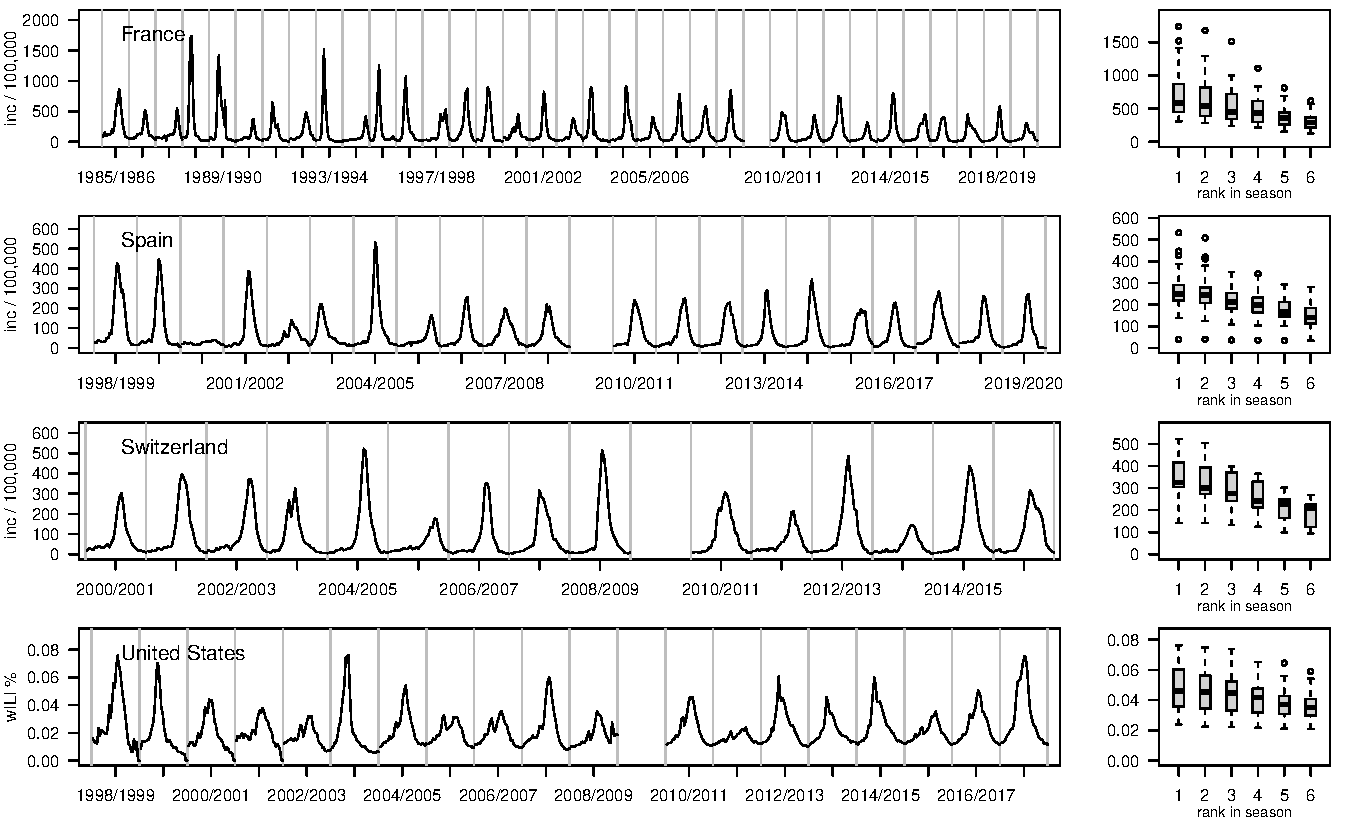
\includegraphics[width=0.9\textwidth]{figure/plot_data.pdf}
\caption{Time series of influenza activity measures in four countries: Weekly ILI cases per 100,000 population in France, 1985--2019; weekly number of confirmed influenza cases per 100,000 population in Spain, 1998--2019; weekly ILI cases per 100,000 in Switzerland, 2000--2016; weekly wILI values in the United States, 1998--2017. Off-season weeks are omitted in the plot, with grey lines delimiting the different seasons.}
\label{fig:data}
\end{figure}

\subsection{Used software}

All analyses were performed using the R language for statistical computing, version 4.0.3 \citep{RCT2020}, in particular using the package \texttt{mem}, version 2.16 \citep{Lozano2020}. Note that the function \texttt{mem::memmodel} provides sufficient flexibility to apply all four approaches (a)--(d) from Section \ref{subsec:simulation_goal}.

\subsection{Results}

Results from our bootstrap simulation study for the four considered countries are shown in Figures \ref{fig:results1} (France, Spain) and \ref{fig:results2} (Switzerland and US). In the first and third colum of each figure we also show the analytical approximations from Section \ref{sec:analytical} as small black dots. To compute these approximations, we just plugged the empirical mean vectors and covariance matrices into equations \eqref{eq:expectation_mu} -- \eqref{eq:expectation_q}. As can be seen, the agreement with the bootstrap results is very good.

In all four countries, the thresholds obtained when using a log transformation as in the MEM are considerably higher than when no transformation is used. Especially in France and Spain, thresholds obtained without the log transformation are clearly too low, as can be seen from the large proportion of seasons classified as very high intensity (around 10\% when using $n = 1$). Applying the log transformation mitigates this to some degree. 

As expected, when letting the number of observations used per season depend on the number of available seasons via $n = 30/m$, average thresholds increase in $m$. As a particularly striking example, the average threshold for high intensity for France when using a log transformation increase from %$q_{0.9} = 834, q_{0.975} = 1158$ for $m = 5, n = 6$ to $q_{0.9} = 1011, q_{0.975} = 1363$ for $m = 10, n = 3$ and $q_{0.9} = 1080, q_{0.975} = 1458$ for $m = 15, n = 2$. For $n = 1$, in which case the estimators can be interpreted as unbiased (Section \ref{sec:analytical}), we obtain averages of $q_{0.9} = 1147, q_{0.975} = 1559$.
834 for $m = 5, n = 6$ to 1011 for $m = 10, n = 3$ and 1080 for $m = 15, n = 2$. For $n = 1$, in which case the estimators can be interpreted as unbiased (Section \ref{sec:analytical}), we obtain an average of 1147. This corresponds to an increase of roughly 35\% relative to the thresholds obtained with $n = 6$. Including historical observations which are not from actual peak weeks thus leads to a considerable lowering of alarm thresholds and will necessarily increase the number of alerts for high and very high influenza activity. As an example, in Spain, applying the MEM with log transformation and $M = 5, n = 6$ leads to 25\% of all seasons exceeding the high threshold and 11\% exceeding the very high threshold. This is obviously rather far from the intended excedance probabilities of 10\% and 2.5\% for the two thresholds.

\begin{figure}
\centering
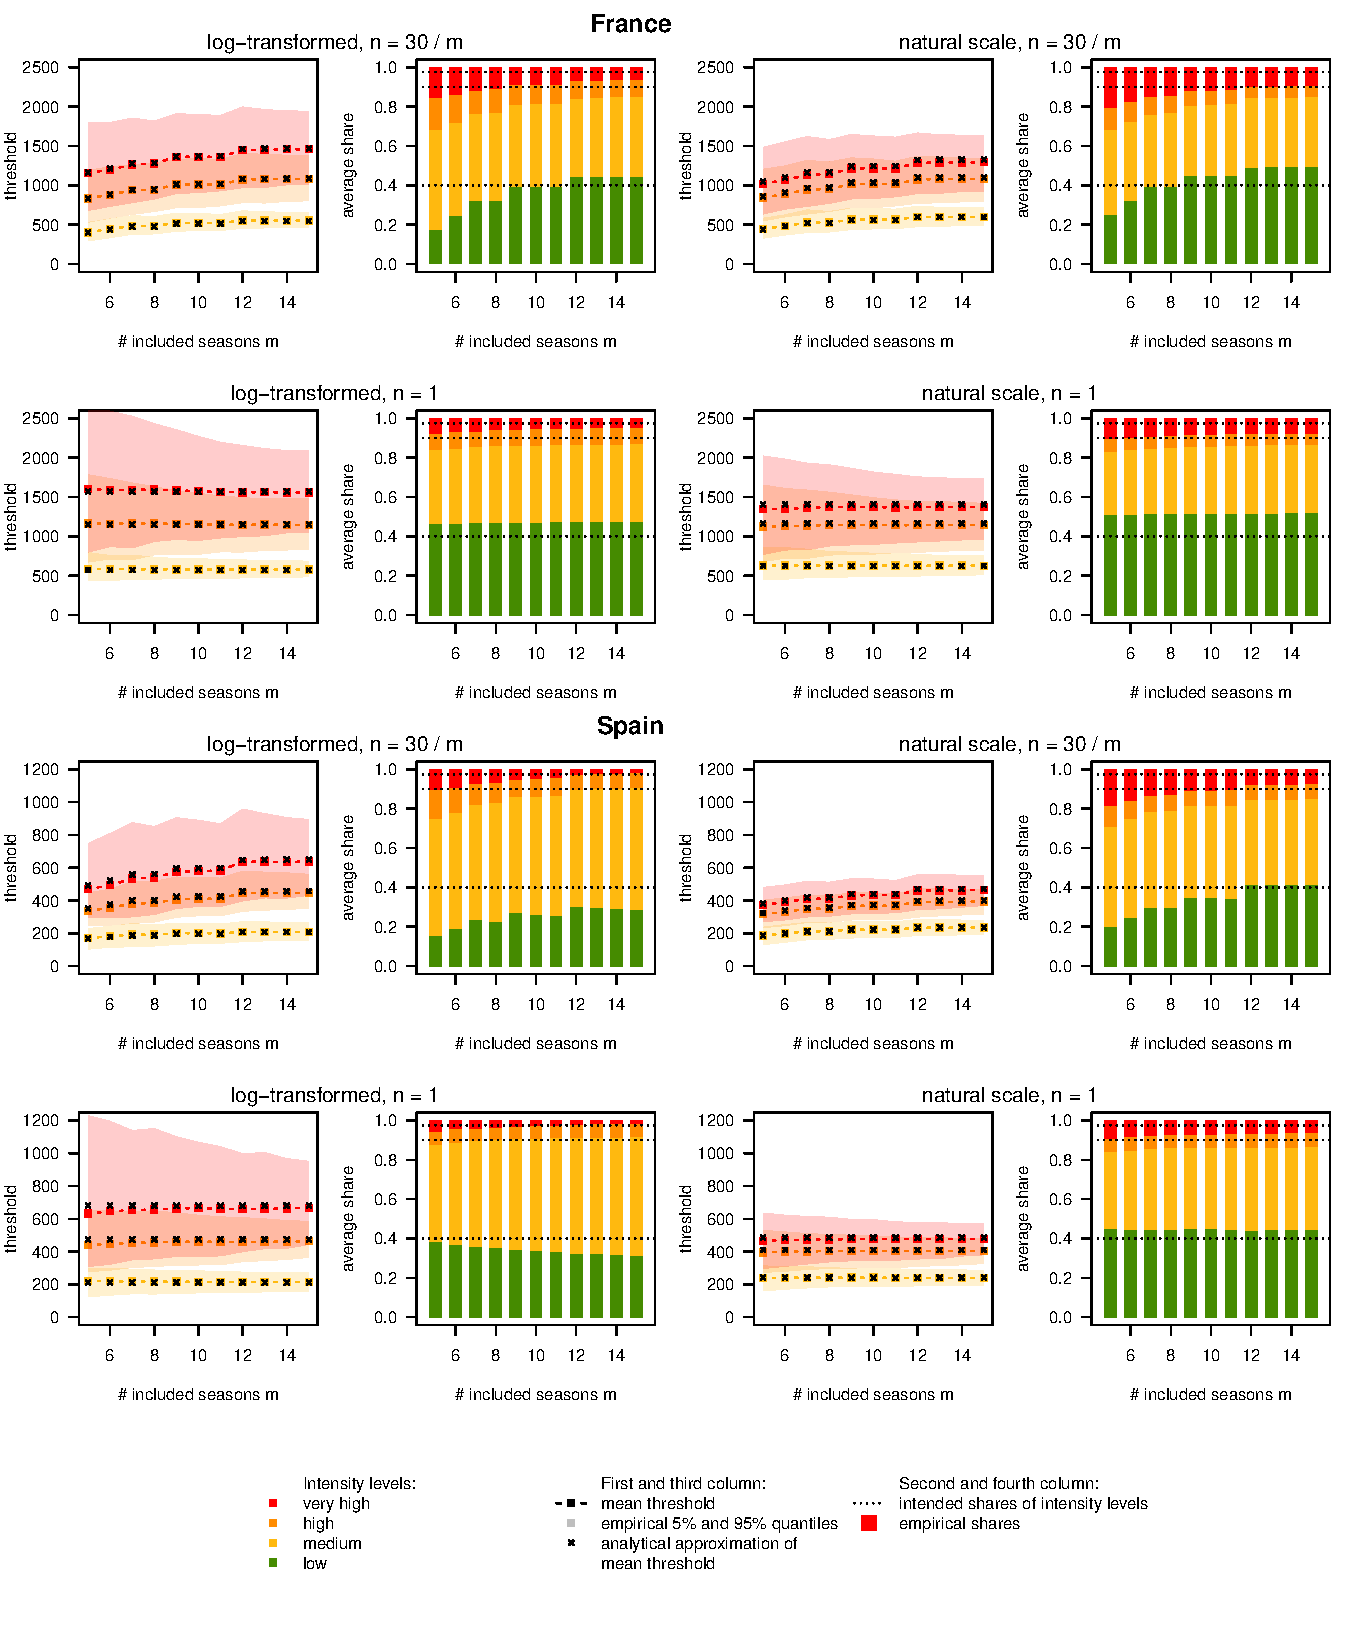
\includegraphics[page=1, width=0.95\textwidth]{figure/plot_results.pdf}
\caption{Results of bootstrap simulation study for France and Spain. First and third column: mean intensity thresholds along with bands delimited by the empirical 5\% and 95\% quantiles. The approximate mean threshold values obtained analytically are marked as little black dots. Second and fourth columns: resulting average shares of seasons classified as low, medium, high and very high intensity (shown as in a stacked barplot).}
\label{fig:results1}
\end{figure}

\begin{figure}
\centering
\includegraphics[page=2, width=0.95\textwidth]{figure/plot_results.pdf}
\caption{Results of bootstrap simulation study for Switzerland and the United States. First and third column: mean intensity thresholds along with bands delimited by the empirical 5\% and 95\% quantiles. The approximate mean threshold values obtained analytically are marked as little black dots. Second and fourth columns: resulting average shares of seasons classified as low, medium, high and very high intensity (shown as in a stacked barplot).}
\label{fig:results2}
\end{figure}

The increase of thresholds as more historical data accumulates is not only a statistical tendency, but occurs with very high probability. Indeed, for all four countries, the probability that the threshold for high intensity increases when using the first ten rather than only the first five years of a sequence was around 90\%. To illutrate this aspect further, we examine the following toy example: We repeat a sequence of five seasons of ILI incidence data from France (2014--2019) four times to obtain a time series of twenty seasons. We then apply the moving epidemic method with log transformation and $n = 30/m$ using the first $m = 5, 6, \dots, 20$ years of data, thus mimicking the development of thresholds as more historical data becomes available. As can be seen from Figure \ref{fig:example_france}, this results in a quite steady increase of thresholds, despite the fact that the data in each five-year block behave exactly the same. For example, season 6 is classified as very high intensity based on seasons 1 through 5, but seasons 11 and 16 are not, even though they are identical to season 6 and the respective data used to construct thresholds follow exactly the same patterns. A similar discrepancy can be observed for season 7, which is classified as medium intensity, while seasons 12 and 17 are marked as low intensity.

\begin{figure}
\center
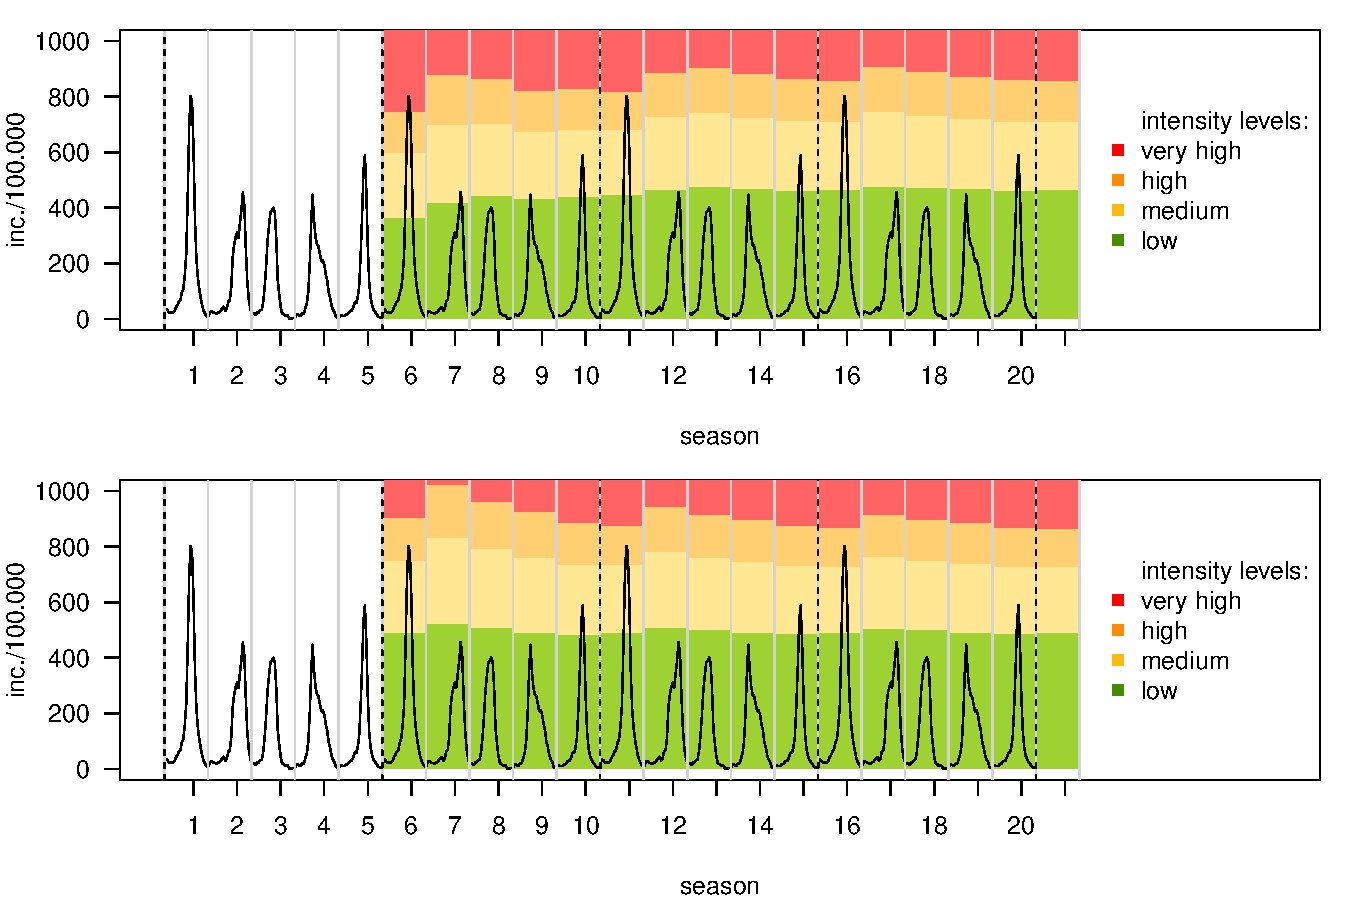
\includegraphics[scale=0.6]{figure/example_france.pdf}
\caption{Toy example to illustrate increasing thresholds as historical data accumulates: Data from France, 2014/2015--2018/2019 are appended three times and thresholds are computed using $m = 5, \dots, 15$ years of training data. The thresholds based on years 1 through $m$ are overlaid with the incidence time series from the $(m + 1)$-th year.}
\label{fig:example_france}
\end{figure}

When just using $n = 1$ irrespective of the number of historical seasons available, the average thresholds and shares of the different categories are more well-behaved also for small $m$. Of course, there is considerable variability in the estimated thresholds. This difficulty, however, is inherent in the problem of estimating a 90\% or 97.5\% quantile based on only 5--10 observations.

\section{Discussion}
\label{sec:discussion}

We provided a statistical assessment of different implementation choices in a simple and widely used framework for the computation of influenza intensity thresholds. We found that using a log transformation to intensity measures prior to the computation of thresholds empirically led to better behaved thresholds with closer to nominal exceedance rates. Concerning the question of how many observations per historical season should be included in the computation of thresholds, we provided analytical arguments and empirical evidence that the common choice $n = 30/m$ leads to too low thresholds when few historical seasons are available. We therefore recommend to adopt $n = 1$ irrespective of the number $M$ of available historical seasons. This is possible using the available implementation in the \texttt{R} package \texttt{mem} and only requires setting \texttt{i.n.max = 1} in the call of the \texttt{memmodel} to override the default value 30/m.

We focused on the computation of influenza intensity thresholds, but the same general arguments apply to the computation of thresholds to determine the onset of a season \citep{Vega2012}. As variability among observations around the season onset may be lower than around the peak the problem may be less severe; we did not assess this empirically as not all our data sets fully covered the off-season.

More sophisticated methods to determine influenza intensity thresholds could be imagined, e.g.\ based on the broad literature on outbreak and anomaly detection \citep{Unkel2012}. However, we think that in practice a simple and interpretable tool with a robust software implementation like the MEM is a good choice. The emergence of a standard approach at the European level and beyond will contribute to improved comparability of results and facilitate the evaluation and refinement of the applied tool. With this work we hope to contribute a statistical perspective on this topic, which can complement public health practitioners' experience from applied analyses.


\section*{Data and code}

Materials to reproduce the presented results are available at \url{https://github.com/jbracher/mem}.


\bibliographystyle{apalike}
\bibliography{bibliography_mem}
\end{document}